The proposed solution technique is designed to be implemented at the PCC(point of common coupling) of a microgrid containing distributed generation and energy storage. An example system can be seen in Fig \ref{fig:system_arch}. Here the ESMS(energy storage management system) is in charge of controlling the battery connected to the grid to get the most cost optimum use of the resources available. The objective of the ESMS is to optimize the use of energy storage under different pricing schemes taking advantage of DG and load forecasting.
\begin{figure}[!htbp]
\centering
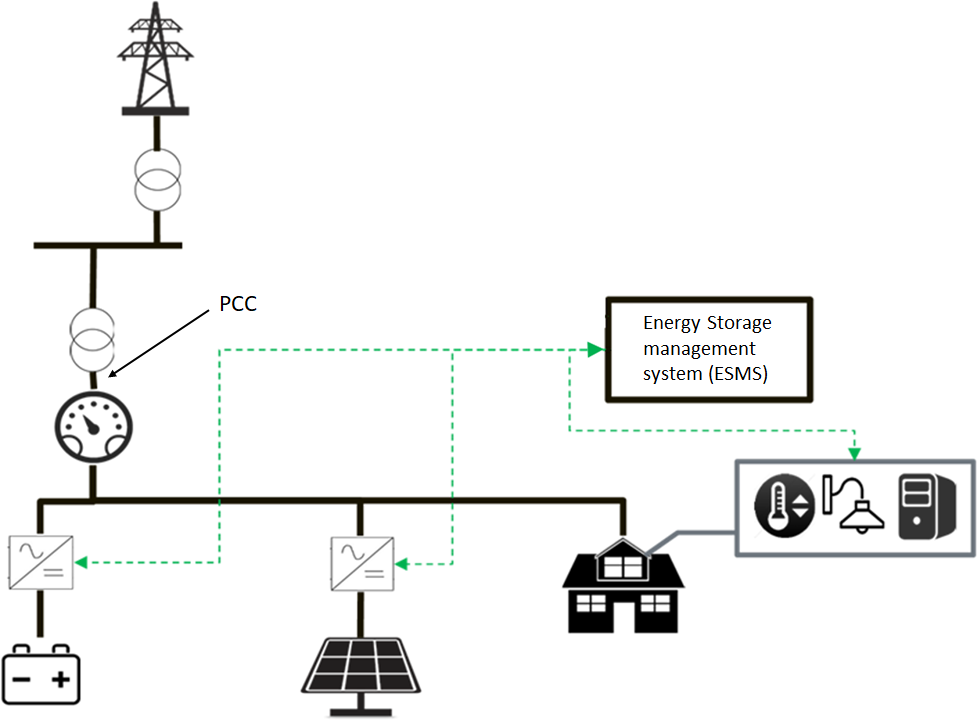
\includegraphics[width=0.45\textwidth]{figs/System_architecture.png}
\caption{Test system architecture}
\label{fig:system_arch}
\vspace{-3mm}
\end{figure}

 Fig \ref{fig:F1_CA} shows the top level architecture of the inputs and outputs of the ESMS. As seen in the figure it will take in the RTP prediction, load prediction and PV prediction as well as the current state of the load, PV generation, and ES. The output of the ESMS is the optimum battery charge and discharge references based on the current and forecasted data.

\begin{figure}[!ht]
    \centering
    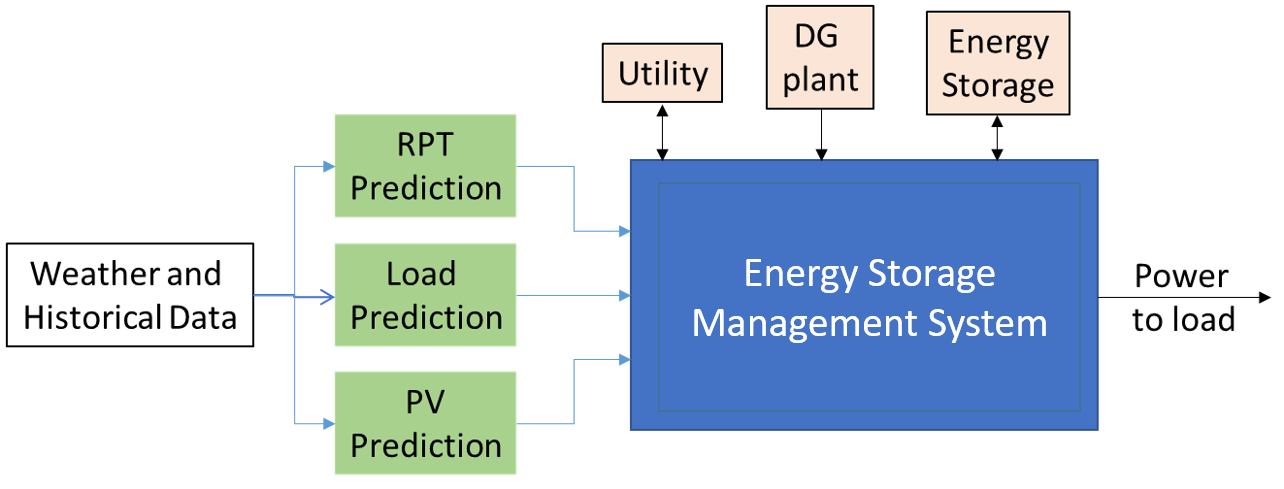
\includegraphics[width = \linewidth]{figs/EMS_FIG.png}
    \caption{Controller top level architecture}
    \label{fig:F1_CA}
\end{figure}

To find the most cost optimum solution based on the current system status and future forecasts the optimization problem is formulated as a graph search problem. To represent the solution space of the problem as a graph the state of charge (SOC) of the ESS is discretized. Also, the time until the prediction horizon is also represented in discrete steps. Fig \ref{fig:F1_Dis} represents a simple example of the discretized solution space.

\begin{figure}[!ht]
    \centering
    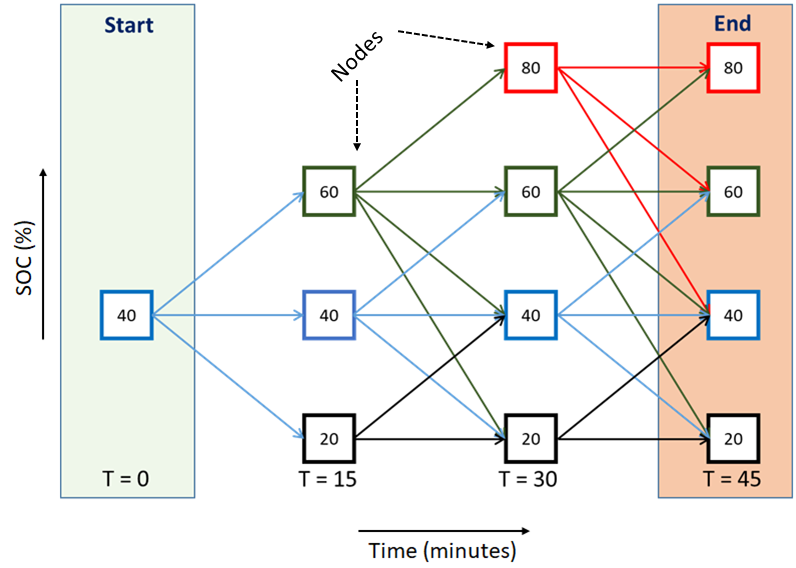
\includegraphics[width = \linewidth]{figs/F1_1_Dis.png}
    \caption{Discretizing solution space}
    \label{fig:F1_Dis}
\end{figure}
Here, the horizontal axis represents time and the vertical axis represents discrete states of charge for the energy storage. In this scenario, it is assumed that the algorithm recalculates the solution every 15 minutes based on available data. The SOC of the ESS is discretized in steps of 20\% and the SOC is limited between 80\% and 20\%. It is also assumed that the ESS can discharge a maximum of 40\% of its maximum charge and charge a maximum of 20\% of its charge in a 15 minute time step. Taking these features into consideration a directed graph is constructed in Fig \ref{fig:F1_Dis}. The colored boxes represent nodes on the graph. The numbers inside the boxes represent the SOC of the ESS at that node. The arrows from the boxes represent all the possible states the ESS can be in in the next time step according to the constraints mentioned before. The arrows are treated as edges of the graph. In this case, the edges are unidirectional.

